%\chapter{Low power wireless network technologies}
\chapter{Technologie pro bezdrátové senzorové sítě}
In the appendix is table where all widely used low power wireless technologies are compared.
This chapter additionally provide a brief description of all these technologies, but the main parameters are only in the table.
All these technologies use license-free ISM bands.


\section{IQRF}
This technology aims to make it easy to implement wireless solutions. It enables peer-to-peer, star and mesh network communication modes. The IQRF alliance provide IQRF transceivers for \$15-20 with a few serial interfaces such as SPI, I2C, UART etc. and they also provide open source SDK which makes it very easy to use IQRF modules. The SDK is based on Java so it's compatible with various platforms such as Linux and Windows
\cite{1} \cite{2} \cite{3} \cite{4}.


\section{Wireless M-bus}
\textit{"Wireless Meter Bus has its origins within the Meter-Bus standards. This is a field bus standard aimed at applications for collecting meter data for gas, electricity, water, etc."} \cite{5}
It supports a few application modes for differing applications.
\begin{itemize}
  \item S1  Unidirectional, data are transmitted only a several times a day.
  \item S2	Bidirectional version of S1.
  \item	T1	Unidirectional transmission of data with a period of a few seconds of minutes.
  \item T2	Bidirectional version of T1.
  \item C1	Unidirectional transmission of bigger amount of data.
  \item C2	Bidirectional version of C1.
\end{itemize}
Usually one M-bus device support only a few of these application modes \cite{5} \cite{6} \cite{7} \cite{8}.


\section{Zigbee}
Zigbee, developed by zigbee alliance is usually used for mesh sensor networks because of its short range. This technology is standardized since 2003, so there is many available nodes at the market by now \cite{10} \cite{11} \cite{12}.

\section{Bluetooth}
Bluetooth has the big advantage, taht it's built in almost every mobile phone, tablet or laptop so there are more options to control the network. The Bluetooth 4.0+ also called BLE (Bluetooth Low Energy) aims to low power wireless sensor networks.
It can be used for point-to-point, broadcast or mesh network topology \cite{13} \cite{14} \cite{15} \cite{16}.


\section{LoRa}
The name LoRa stands for "Long Range" wireless communication with low data rate and power consumption. The protocol enables to modify SF which affects the communication range and data rate. The \ref{fig:loraSF} shows this dependence.

\begin{figure}[!h]
    \centering
    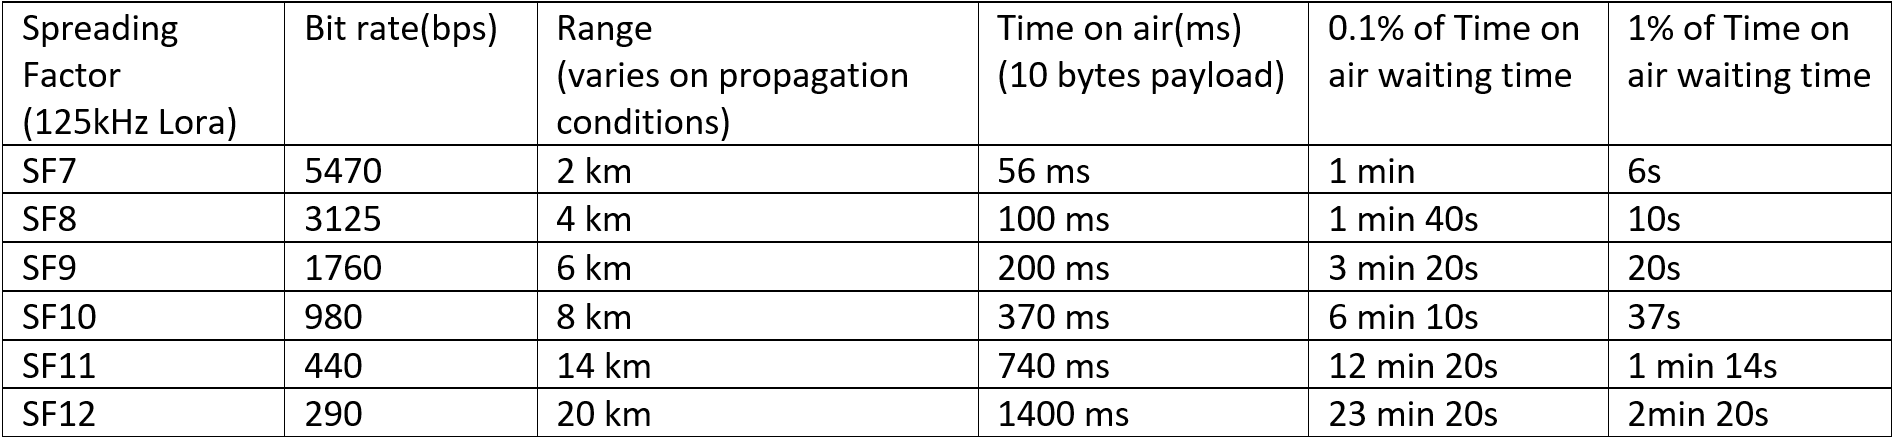
\includegraphics[width=1\textwidth]{spreading_factor_lorawan_2017-07-29}
    \caption{LoRa spread factor options \cite{24}}
    \label{fig:loraSF}
\end{figure}

This technology is very attractive for its long range capability and easy to connect nodes. It's complicated to build a full-capacity gateway which is capable of receiving packets at all frequency channels and SF in parallel. The transceiver for this application costs about \$130. Although it's also possible to build single-channel gateway which is way too cheaper, but it can receive packets at only one frequency channel and SF at once \cite{17} \cite{18} \cite{19} \cite{20} \cite{21} \cite{22} \cite{23} \cite{24}.


\section{Sigfox}
This technology focuses on short message and long range communication applications \cite{25} \cite{26}.


\section{Z-Wawe}
Z-Wave is intended for wireless connectivity for all possible smart home products, controlled by PC, phone, voice, etc. It's based on mesh network topology so every non-battery powered device works as a router to enhance the network range so the more devices are connected in one network, the stronger the network is \cite{27} \cite{28}.


\section{Thread}
This technology based on IPv6 was developed for home network controlled by smartphone, tablet or PC \cite{29} \cite{30} \cite{31}.


\section{RPMA}
The "Random Phase Multiple Access" developed by Ingenu designed for M2M and IoT applications \cite{32} \cite{rpma_ublox} \cite{34}. \textit{"RPMA has been deployed for the Machine Network, but can also be rolled out as a private network installation. It is highly suitable for regions, where the rollout of 3GPP LPWA technologies is lagging, where cellular coverage is generally weak, or where users would like to exert full control over their network deployments."}\cite{rpma_ublox}


